\subsubsection{Hỏi đáp thông tin công tác xã hội qua Chatbot}
\begin{figure}[H]
    \centering
    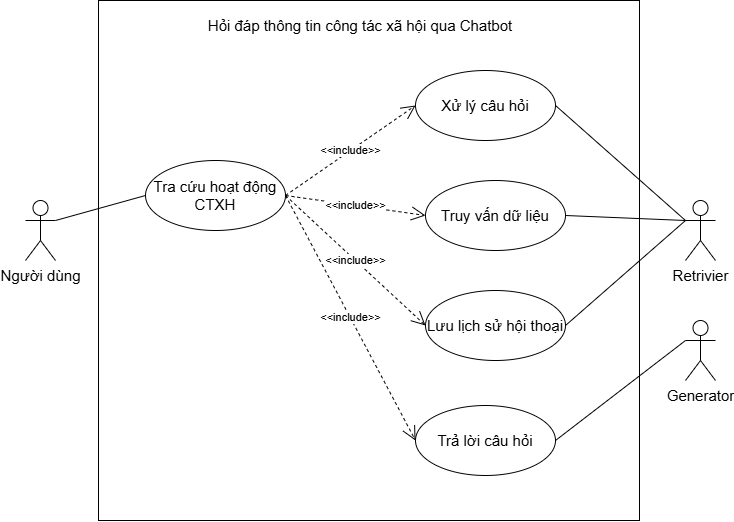
\includegraphics[width=1.0\linewidth]{Images/use-case-diagram/UC09_chatbot_usecase.drawio.png}
    \vspace{0.3em}
    \caption{UC09 - Tra cứu hoạt động Công tác xã hội qua Chatbot}
    \label{fig:uc01-usecase}
\end{figure}
\newpage
%--------------- Bảng mô tả Chatbot -----------------------------
\renewcommand{\arraystretch}{1.3}
\begin{longtable}{|m{0.25\textwidth}|m{0.75\textwidth}|}
 \hline

\textbf{Use-case Name} & \textbf{UC09. Tra cứu hoạt động Công tác xã hội qua Chatbot} \\ \hline
\endfirsthead

\hline
\textbf{Use-case Name (tiếp)} & \textbf{UC09. Tra cứu hoạt động Công tác xã hội qua Chatbot} \\ \hline
\endhead

% ===== Nội dung bảng =====
\textbf{Actors} 
& \begin{itemize}[label=--]
    \item Người dùng
    \item Retriever (Hệ thống truy xuất)
    \item Generator (Hệ thống tạo nội dung)
\end{itemize} \\ 
\hline

\textbf{Description} 
& Người dùng gửi câu hỏi về các hoạt động Công tác xã hội (CTXH). 
Hệ thống Chatbot thực hiện xử lý ngôn ngữ tự nhiên, truy xuất dữ liệu phù hợp từ cơ sở dữ liệu kiến thức và tạo ra câu trả lời tự nhiên để phản hồi cho người dùng, đồng thời lưu lại lịch sử cuộc trò chuyện nhằm duy trì ngữ cảnh hội thoại \\ 
\hline

\textbf{Trigger} 
& Người dùng nhập và gửi một câu hỏi liên quan đến hoạt động CTXH vào giao diện Chatbot. \\ 
\hline

\textbf{Pre-Conditions} 
&
\begin{itemize}[label=--]
    \item Hệ thống Chatbot đang hoạt động
    \item Cơ sở dữ liệu kiến thức về CTXH đã được chuẩn bị và sẵn sàng
    \item Các dịch vụ AI LLM (sử dụng ở Retriever và Generator) đang ở trạng thái trực tuyến
\end{itemize}
\\ 
\hline

\textbf{Post-Conditions} 
&
\begin{itemize}[label=--]
    \item Người dùng nhận được câu trả lời phù hợp với câu hỏi đã gửi
    \item Lịch sử hội thoại được ghi nhận vào hệ thống
    \item Trạng thái phiên hội thoại được cập nhật để sẵn sàng cho câu hỏi tiếp theo
\end{itemize}
\\ 
\hline

\textbf{Normal Flow} 
&
\begin{enumerate}
     \item Người dùng gửi câu hỏi về hoạt động CTXH.
    \item Hệ thống thực hiện xử lý câu hỏi (phân tích ý định và nội dung).
    \item Hệ thống phối hợp với \textit{Retriever} để truy vấn dữ liệu từ cơ sở dữ liệu kiến thức.
    \item Hệ thống lưu lịch sử hội thoại nhằm duy trì ngữ cảnh.
    \item Hệ thống phối hợp với \textit{Generator} để tổng hợp thông tin và tạo câu trả lời.
    \item Hệ thống trả lời câu hỏi cho người dùng.
\end{enumerate}
\\ 
\hline

\textbf{Alternative Flow} 
& Ở bước 3:
\begin{itemize}
    \item \textbf{3a.} Hệ thống không truy xuất được dữ liệu phù hợp. Hệ thống thông báo không tìm thấy thông tin và gợi ý người dùng đặt câu hỏi khác.
\end{itemize}
\\ 
& Ở bước 2:
\begin{itemize}
    \item \textbf{2a.} Hệ thống xác định câu hỏi không liên quan đến CTXH. Hệ thống từ chối trả lời và hướng dẫn người dùng về các chủ đề được hỗ trợ.
\end{itemize}
\\
\hline

\textbf{Exception} 
& Ở bước 3 hoặc 5:
\begin{itemize}
    \item \textbf{3a. hoặc 5a.} Lỗi kết nối dịch vụ AI khiến hệ thống không thể kết nối tới Retriever hoặc Generator. Hệ thống hiển thị thông báo: \textit{``Dịch vụ đang gặp sự cố, vui lòng thử lại sau.''}
\end{itemize}
\\
\hline
\caption{Bảng mô tả Use Case UC09 - Tra cứu hoạt động Công tác xã hội qua Chatbot}
\end{longtable}
